\documentclass[journal,12pt,twocolumn]{IEEEtran}

\usepackage{setspace}
\usepackage{gensymb}

\singlespacing


\usepackage[cmex10]{amsmath}

\usepackage{amsthm}

\usepackage{mathrsfs}
\usepackage{txfonts}
\usepackage{stfloats}
\usepackage{bm}
\usepackage{cite}
\usepackage{cases}
\usepackage{subfig}

\usepackage{longtable}
\usepackage{multirow}

\usepackage{enumitem}
\usepackage{mathtools}
\usepackage{steinmetz}
\usepackage{tikz}
\usepackage{circuitikz}
\usepackage{verbatim}
\usepackage{tfrupee}
\usepackage[breaklinks=true]{hyperref}
\usepackage{graphicx}
\usepackage{tkz-euclide}

\usetikzlibrary{calc,math}
\usepackage{listings}
    \usepackage{color}                                            %%
    \usepackage{array}                                            %%
    \usepackage{longtable}                                        %%
    \usepackage{calc}                                             %%
    \usepackage{multirow}                                         %%
    \usepackage{hhline}                                           %%
    \usepackage{ifthen}                                           %%
    \usepackage{lscape}     
\usepackage{multicol}
\usepackage{chngcntr}

\DeclareMathOperator*{\Res}{Res}

\renewcommand\thesection{\arabic{section}}
\renewcommand\thesubsection{\thesection.\arabic{subsection}}
\renewcommand\thesubsubsection{\thesubsection.\arabic{subsubsection}}

\renewcommand\thesectiondis{\arabic{section}}
\renewcommand\thesubsectiondis{\thesectiondis.\arabic{subsection}}
\renewcommand\thesubsubsectiondis{\thesubsectiondis.\arabic{subsubsection}}


\hyphenation{op-tical net-works semi-conduc-tor}
\def\inputGnumericTable{}                                 %%

\lstset{
%language=C,
frame=single, 
breaklines=true,
columns=fullflexible
}
\begin{document}


\newtheorem{theorem}{Theorem}[section]
\newtheorem{problem}{Problem}
\newtheorem{proposition}{Proposition}[section]
\newtheorem{lemma}{Lemma}[section]
\newtheorem{corollary}[theorem]{Corollary}
\newtheorem{example}{Example}[section]
\newtheorem{definition}[problem]{Definition}

\newcommand{\BEQA}{\begin{eqnarray}}
\newcommand{\EEQA}{\end{eqnarray}}
\newcommand{\define}{\stackrel{\triangle}{=}}
\bibliographystyle{IEEEtran}
\providecommand{\mbf}{\mathbf}
\providecommand{\pr}[1]{\ensuremath{\Pr\left(#1\right)}}
\providecommand{\qfunc}[1]{\ensuremath{Q\left(#1\right)}}
\providecommand{\sbrak}[1]{\ensuremath{{}\left[#1\right]}}
\providecommand{\lsbrak}[1]{\ensuremath{{}\left[#1\right.}}
\providecommand{\rsbrak}[1]{\ensuremath{{}\left.#1\right]}}
\providecommand{\brak}[1]{\ensuremath{\left(#1\right)}}
\providecommand{\lbrak}[1]{\ensuremath{\left(#1\right.}}
\providecommand{\rbrak}[1]{\ensuremath{\left.#1\right)}}
\providecommand{\cbrak}[1]{\ensuremath{\left\{#1\right\}}}
\providecommand{\lcbrak}[1]{\ensuremath{\left\{#1\right.}}
\providecommand{\rcbrak}[1]{\ensuremath{\left.#1\right\}}}
\theoremstyle{remark}
\newtheorem{rem}{Remark}
\newcommand{\sgn}{\mathop{\mathrm{sgn}}}
\providecommand{\abs}[1]{\vert#1\vert}
\providecommand{\res}[1]{\Res\displaylimits_{#1}} 
\providecommand{\norm}[1]{\Vert#1\rVert}
%\providecommand{\norm}[1]{\lVert#1\rVert}
\providecommand{\mtx}[1]{\mathbf{#1}}
\providecommand{\mean}[1]{E[ #1 ]}
\providecommand{\fourier}{\overset{\mathcal{F}}{ \rightleftharpoons}}
%\providecommand{\hilbert}{\overset{\mathcal{H}}{ \rightleftharpoons}}
\providecommand{\system}{\overset{\mathcal{H}}{ \longleftrightarrow}}
	%\newcommand{\solution}[2]{\textbf{Solution:}{#1}}
\newcommand{\solution}{\noindent \textbf{Solution: }}
\newcommand{\cosec}{\,\text{cosec}\,}
\providecommand{\dec}[2]{\ensuremath{\overset{#1}{\underset{#2}{\gtrless}}}}
\newcommand{\myvec}[1]{\ensuremath{\begin{pmatrix}#1\end{pmatrix}}}
\newcommand{\mydet}[1]{\ensuremath{\begin{vmatrix}#1\end{vmatrix}}}
\numberwithin{equation}{subsection}
\makeatletter
\@addtoreset{figure}{problem}
\makeatother
\let\StandardTheFigure\thefigure
\let\vec\mathbf
\renewcommand{\thefigure}{\theproblem}
\def\putbox#1#2#3{\makebox[0in][l]{\makebox[#1][l]{}\raisebox{\baselineskip}[0in][0in]{\raisebox{#2}[0in][0in]{#3}}}}
     \def\rightbox#1{\makebox[0in][r]{#1}}
     \def\centbox#1{\makebox[0in]{#1}}
     \def\topbox#1{\raisebox{-\baselineskip}[0in][0in]{#1}}
     \def\midbox#1{\raisebox{-0.5\baselineskip}[0in][0in]{#1}}
\vspace{3cm}
\title{ASSIGNMENT-2}
\author{UNNATI GUPTA}
\maketitle
\newpage
\bigskip
\renewcommand{\thefigure}{\theenumi}
\renewcommand{\thetable}{\theenumi}
Download all python codes from 
\begin{lstlisting}
https://github.com/unnatigupta2320/Assignment-2/tree/master/codes
\end{lstlisting}
%
and latex-tikz codes from 
%
\begin{lstlisting}
https://github.com/unnatigupta2320/Assignment-2/tree/master
\end{lstlisting}
%
\section{Question No. 2.36}
Construct a quadrilateral MIST where $MI = 3.5, IS = 6.5, \angle M = 75 \degree, \angle I = 105 \degree$ and $\angle S = 120 \degree$.
%
\section{SOLUTION}
For this quadrilateral MIST we have,
\begin{align}
\angle M +\angle I = 75\degree + 105\degree =180\degree,
\end{align}
$ \implies MT \parallel IS (\because \text {MI being the transversal})$
\\
As, sum of adjacent angle on same side is $180\degree$ only when lines are parallel.
\begin{enumerate}
    \item Now, considering ST as another transversal on parallel lines MT and IS then$\angle S$ and $\angle T $being on same side of transversal, we get
\begin{align}
&\implies \angle S + \angle T = 180\degree,
\\
&\implies \angle T = 60\degree\label{eq1}
\end{align}
 \item Now taking sum of all the angles given and \eqref{eq1}  \text{we get}
\begin{align}
\angle M + \angle I +\angle S +\angle T =360\degree
\end{align}
So construction of given quadrilateral is possible as sum of all the angles is equal to $360\degree$.
\\
 \item Now,Using cosine formula we can find SM:
\begin{multline}
\implies {\norm{\vec{S}-\vec{M}}^2}=
\\
{\norm{\vec{M}-\vec{I}}^2}+ \norm{\vec{I}-\vec{S}}^2-2\times\norm{\vec{M}-\vec{I}} \times \norm{\vec{I}-\vec{S}}\cos{I}
\end{multline}
\begin{align}
&\implies SM=8.14
\end{align}
\item Also,using sine formula in $\triangle MIS$,we have
\begin{align}
\frac{{\sin M}}{m} = \frac{{\sin I}}{i} = \frac{{\sin S}}{s}
\end{align}
\begin{align}
\angle M=\arcsin 0.7713;
\\
\angle M= 50.47 \degree ;
\end{align}
\item Now,polar coordinates of vertex S of $\triangle MIS$ be
\\$(SM \cos M,SM\sin M)$, we get
\begin{align}
S(8.14\times \cos50.47 ,8.14\times \sin50.47)
\\
\implies S(5.18,6.27)
\end{align}
\item Using sine formula in $\triangle MTS$,we get
\begin{align}
\angle TMS= 24.53\degree
\end{align}
\item Considering the polar coordinates of T of $\triangle MTS$ and solving we get,
\begin{align}
T(2.42,9.03)
\end{align}
    \item Now, we have the coordinate of vertices M,I,S,T as M(0,0); I(3.5,0); S(5.18,6.27);T(2.42,9.03);
    \item We can construct the quadrilateral.On constructing the given quadrilateral we, get:
\end{enumerate}
\numberwithin{figure}{section}
\begin{figure}[!ht]
\centering
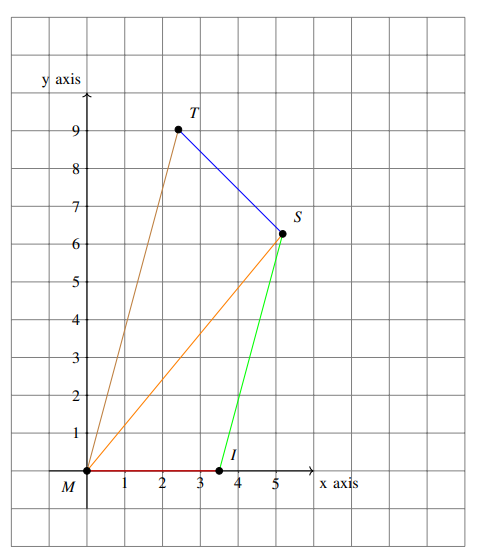
\includegraphics[ width=\columnwidth, height=7 cm]{MISTQuadilateral.PNG}
\caption{Quadrilateral MIST}
\label{fig:Quadrilateral MIST}	
\end{figure}
\end{document}